\documentclass[12pt]{article}
\usepackage[utf8]{inputenc}
\usepackage{amsmath}
\usepackage{graphicx}
\usepackage{subfigure}
\usepackage{color}
\usepackage{amssymb}
\usepackage{appendix}
\usepackage{tabularx}
\usepackage{cite}
\begin{document}
\title{Build a Web Application System for Anti-epidemic Purpose}
\date{}
\maketitle
\begin{center}
\textrm{Name: Yiran Dai}\\
\end{center}
\begin{center}
\textrm{Student ID: 1847094}\\
\end{center}
\begin{center}
\textrm{Study Programme: BSc Computer Science FT}\\
\end{center}
\begin{center}
\textrm{Supervised By: Dr Rami Bahsoon}\\
\end{center}
\begin{center}
\textrm{Word Count: 9624 (Via Overleaf)}\\
\end{center}
\parbox[t][2cm][b]{\textwidth}{
\begin{center}{\large\textrm May 2021} \end{center} }
\maketitle
\thispagestyle{empty}
\newpage
\thispagestyle{empty}
\begin{abstract}
In the year 2020, the world has faced an unexpected worldwide epidemic, the COVID-19, a disease caused by a new coronavirus that was first identified in December 2019. This kind of disease can be spread from person to person during close contact and air transmission fast and easily. Since developing an efficient vaccine need time to research, therefore, the best way to stop the virus spread beside the vaccine at the first time is to do the laboratory test and reduce the personal contact with each other as much as possible. This project aims to develop a disease diagnosis and self-report, management system mainly faced to the University students who are currently self-isolating which let them can report and track their daily health status to ensure whether they are healthy or need medical help and further self-isolated, at the backstage of the system it will be able to store, manage and view all the user’s health information to do the meaningful data analysis and manage the human resources to avoid the virus will be further spread and infect in the public territory. 
\end{abstract}
\newpage
\thispagestyle{empty}
\tableofcontents
\newpage
\setcounter{page}{1}
\section{Introduction}
In the University, illness and physical health issues will highly affect the performance of students. There are several reasons, first, they may not have enough vigor and attention to study new contents, finish their assignments, review their lectures instead of they need more time to recovery and rest since they are ill, therefore, their progress will be slow down and their plan will fall behind, this will cause time management problems, if a student can not or unable to manage their time properly, it is common to see that they finish their works until the last minutes before the deadlines, give more stressful, moreover, they may entirely miss the deadlines of their assignments and can not finish their works on time or they can not be able to attend their examinations. Thus, their study outcomes will be influenced both in the result, grade, and the understanding of knowledge. In some cases, this will mislead the evaluation of a student outcome and wrongly reflect the students’ study level. From the perspective of students, this may also damage their self-confidence and even raise mental health issues. 
\\
\\The coronavirus will cause serious health issues in the University if we do not treat it properly. In-person lectures, using the University facilities such as the library, laboratory, study rooms, coffee shop, or meeting with each other, etc, those are potentially high-risk activities that will let the virus keep spread, the students and staff members will face a higher probability to be infected by the coronavirus. For safety reasons, also due to the limited medical resources, so far the best way for University that can keep teaching by reducing the danger and avoid the virus keep spread is to work remotely, deliver the contents and teaching sessions online.
\\
\\However, work remotely and teaching online will face multiple challenges such as network connection issues, distraction during the online sessions, and also we may doubt the teaching quality between offline teaching and online teaching. Hence, to help students return to the University in safety under the appropriate social policy, provide a system that can track, store, and do the meaningful and helpful data statistics of the students’ daily health status will be developed in this project. This system will also help the university staff members sort the students who meet the health conditions back to the University and the students who need medical help or self-isolated to make sure everyone will study and work in safety.
\section{Literature Review}
\begin{itemize}
\item\textbf{Evolution of Healthcare Applications}
\\As evolved of the science and technology, the number of advance electronic device users is growing rapidly \cite{charland2011mobile}, the functionalities on those devices can be performed become more helpful and efficient by install various software and use different applications, they more like a daily assistant not just machines nowadays, one of the functions on the smart devices are including healthcare. Let us back to ten years ago, in April 2011, MEDLINE is running a project, they were searched the articles and thesis that discussed the design, development, evaluation, and the smartphone-based healthcare software for the professionals in healthcare or the patients \cite{mosa2012systematic}. Based on the research result from MEDLINE, in the total of 83 applications were documented, 57 of them focusing on disease diagnosis, the rest of the applications are focusing on the other different research areas in medical and healthcare such as medical calculators, training or for other specific usages. The disease diagnosis has been reported as the most useful applications by professionals in healthcare and the patients \cite{mosa2012systematic}.
\\
\\The internet and the web technology has keep evolved from ages ago, start from an academic research project to "The Internet of Things (IoT)" nowadays, to making the devices be able to communicate and share information with each other through the cloud, it can let the applications to collect, record and analyse the data quickly and accurately \cite{kulkarni2014healthcare}. During the current epidemic situation, we may realize the importance of report the health status in time if any symptoms have shown up, take appropriate medical treatment, and observation before the virus has started to contaminate any further is extremely important. However, it is rare to have a specific platform for us to report and record such data, there various applications have been used to record the information depend on the different institutions including ``Google Sheets''or ``Microsoft Excel'', two famous applications that aim to manage the data. They are powerful and steady without doubt, but they have the same point is they are not initially designed for epidemic situations or health purposes. Therefore, various features may produce extra study costs for users that not familiar with them before \cite{vora2009web}. So, what if we build a lightly, succinct application only for health purposes.
\\To develop an application from beginning, there are significant parts should take into account both in the software engineering and web technology.
\item\textbf{Applications Design Patterns}
\\Alternatively, when we want to design and implement a new application, there are several factors that need to be considered about including the user interaction, maintainability, capabilities, application performance, potential problems, which platform and device that the application will support \cite{vora2009web}. In the rest of the report, the different types of applications will split into native applications and web applications in general.
\item\textbf{Interaction and User Interface Design}
\\User-interaction is always related to the usability of a software or an application product, in the application development, a well-designed user interface will show to users the entrance of each function directly and clearly, also enhance the usability of an application \cite{Oppermann2002}, lack of the UIs design will increase the error rates, give the higher study costs, a hard, complexity usage application will even cause the stress or other negative induced emotions to the users \cite{Oppermann2002}, therefore, a clear, well-organized user interface design will significantly reduce the negative effects of application usage, increasing the ease of usability.
\item\textbf{Software Maintainability}
\\Another important role when we evaluate an application is to see the maintainability of the application, whether it is easy or able to maintain, how much sources (time, money, equipment) it will cost. Most of the applications will need to keep update in order to let them constantly growing and evolving \cite{4221621}, fixed the bugs to let the application work as plan and more stable, thus, write the codes and functions well organized and logically is an ideal way to simplify debugging process and fix the bugs in the test stage or in the future, if the codes are confusing, without proper logic and statements inside the application, it will spend much more time work on to find out, locate and fix the bugs, sometimes it will affect the schedules of the development. Fixing bugs is a common process in application development, ideally, it will cost 5-10 percentages of the initial project development time \cite{bennett2000software}.
\\
\\As the application keeps growing, it is not difficult to find out new ideas and add new features to the application, therefore, implementing a new function is needed. Whether the application can be expanded without a system crash or it will rise some sort of critical issues; does the application can be further modified in order to adapt to different circumstances in the future; the functionality of other features also should work properly after the new function added. Those are some significant points that we need to think about and evaluate before and during the application development. Normally, the cost of add and test a new functionality will estimate the same as initial development \cite{bennett2000software}.
\item\textbf{Development Decision Making}
\\The client used for the students, as the user-client should make the application as an efficient health care application, to let the users be able to report and submit their personal information, daily health status also can self-diagnose to help them decide whether they need further medical help. The manage-client for the staff members in the University to let them view and manage the data collected from students. Design the application as a native app will improve the capabilities and the performance of the application compared with a web application \cite{charland2011mobile}. However, if design an application as a native app, the platforms that the application will support must be considered about, more platforms need to support means more workload and time needed. Consider the special epidemic circumstance, the students may currently stay in different places around the world, they may also face different anti-epidemic policies, it probably not easy for students to find a supported device in order to use the system in some cases since this system will be widely used for all the students in order to arrange them return to the University. 
\item\textbf{Reachability}
\\Based on the result of weighing the pros and cons between a native application and a web application, a web application will be a wiser choice in the current circumstance. A native application always needs to download and set up on the support platform, obviously, that will cause extra cost. A web application does not need to be downloaded and set up, by using modern web technology, HTML5 and JavaScript can deliver suitable functionality, data transfer to any web-capable devices. Simply provide the internet connection and fetch the web page sources as required so it can perform the functionality, this can easily be done on multiple kinds of personal electronic devices such as smartphones, tablets, laptops, or desktops without platform support issues. Until February 2021, 85 percents of the smart devices support the full HTML5 and JavaScript by using the WebKit, Blink, or Firefox Quantum-based browsers \cite{statcounter2021}.
\item\textbf{Data Management}
\\Moreover, only collect the data from users (in this report is students) is not sufficient. We always need a warehouse to store our goods, therefore, in computer science, we need a database to store our data in order to let the staff members in the University can manage, doing the data statistics easily. A database can store the structured information, data electronically in the computer system, usually along with a database management system (DBMS) in order to control the database, a database associated with a database management system (DBMS) called a database system \cite{hick2006database}. The inception of databases start in the early 1960s \cite{letkowski2015doing}. The evolved of database start at the hierarchical database, this kind of database relied on a tree data structure and only allowed one-to-many relationship, also there is another database called the network database which has more flexible model allowed multiple relationships. However, those systems that were designed early are not quite flexible, the relational databases became more and more popular in the 1980s, along with object-oriented databases in the 1990s. After then, more different kinds of databases have been invented such as NoSQL databases, cloud databases, self-driving databases \cite{olle2003database}.
\item\textbf{Introducing MySQL}
\\SQL, represent as ``Structured Query Language'' is one of the programming languages used to query, manipulate, define the data, do the access control for the relational databases \cite{beynon2004database}. MySQL is an open-source, widely used database management system based on SQL first invented in 1995, Sweden now belongs to the Oracle Corporation \cite{letkowski2015doing}. Also, MySQL was designed and optimized for the web applications and be able to run on any platforms, therefore, MySQL will be the database management system used to store the data in the development and further methodology will be described in the next.
\end{itemize}
\section{Methodology}
\subsection{Design Analysis}
Based on the summary from the literature review, requirements were identified to build the functional application, more specifically, which techniques will be applied in the design and built phase. One of the featured requirements is this application should perform properly with fewer extra components set up and installed as possible, also, there should less bothering with system compatibility constraints. Therefore, to design a web application, it is reasonable to use the HTML, CSS, and JavaScript techniques to write the front-end of the application in order to implement the user interface and functional interaction with users. Another requirement is beside the user client for the students, the application should also have another client as the manage client, the manage client should collect, gathering and store the necessary data and information from each user client for further meaningful data analysis and data statistics. On the basis of the compatibility and popularity, using MySQL as the database management system to manage the data and use the Java Data Base Connectivity as (JDBC) interact with the database, give a shortcut to access, fetch the data to the application with Java programming language at the back-end.
\\
\\In the next section, the featured requirements of the application will further describe and explain in detail. 
\subsection{Requirements}
This section will discuss the requirements specified, the requirements will be spilt into functional requirements and non-functional requirements, by considering this application has multiple clients for the different usage, the functional requirements and non-functional requirements will discuss as in different usage view separately.
\subsubsection{Functional Requirements}
Based on the different user roles will use this application in a specific way and different functionality, we can divide the requirements into smaller pieces by the user roles. Currently, there are mainly have two different user roles and usages for this application. They are:
\begin{itemize}
\item\textbf{General Users}
\\The general users represent as ``Students Users'' in this scenario, typically, the users are the students who are willing or need to return to the University, therefore, they have to submit their daily health status and necessary information that will help the University to prevent the virus spread around the University area, the requirements for the general users will discuss which elements and functions that students can submit required information via the general user client.
\item\textbf{Managers}
\\The Managers represent as ``The person who will manage the collected data'', generally, they are University staffs or administrator who has the right permission and will be able to view the information collected from each student via the manage client in order to do the further data analysis.
\end{itemize}
\subsubsection{Functional Requirements for the General Users}
For the general user client as general users:
\\$\mathbf{(FR1.)}$ The client must create a unique user id (UID) and generate a token to identify each user.
\\$\mathbf{(FR2.)}$ The client must have a portal to let users edit and update their personal information that need to be collected.
\\$\mathbf{(FR3.)}$ The client must give a response and tell the user whether the modify has succeed or failed after each time the user has edited or updated their personal information.
\\$\mathbf{(FR4.)}$ The client must have a portal to let users be able to submit daily health status.
\\$\mathbf{(FR5.)}$ The client must give a response and tell the user whether their daily health data has been sent to the manage client.
\\$\mathbf{(FR6.)}$ The client must send the requested data after each submission via server to the database in order to make sure the data is up to date.
\\$\mathbf{(FR7.)}$ The client shall login with correct username and password combination.
\\$\mathbf{(FR8.)}$ The user shall be able to create a new account in order to login to the system.
\\$\mathbf{(FR9.)}$ The user password shall be future changed and updated by user.
\\$\mathbf{(FR10.)}$ The client shall give several reasonable healthy advice after each submission.
\\$\mathbf{(FR11.)}$ The client shall give the time counting notification for their remaining isolation days.
\\$\mathbf{(FR12.)}$ The client may indicate health status level notification display as different color.
\\$\mathbf{(FR13.)}$ The client may provide health advice, suggestions or news.
\\$\mathbf{(FR14.)}$ The client may display the history of the submission.
\\$\mathbf{(FR15.)}$ The client may support register and log in with University email addresses, accounts in order to reduce the potential accounts management issues in the future.
\subsubsection{Functional Requirements for the Managers}
For the manage client as managers:
\\$\mathbf{(FR1.)}$ The client must access with administration username and password combination who has the right permission.
\\$\mathbf{(FR2.)}$ The client must make a valid connection with database in order to fetch the data into the system.
\\$\mathbf{(FR3.)}$ The client must be able to view the data that initial collected from each user client.
\\$\mathbf{(FR4.)}$ The client must update and refresh the data after receive each new submission or update from the user client.
\\$\mathbf{(FR5.)}$ The client shall have a data visualize system in order to filter and visualize the data depend on the different filter criteria.
\\$\mathbf{(FR6.)}$ The data visualize system should perform the data as a chart.
\\$\mathbf{(FR7.)}$ The client shall have the permission to change the user client password for each user.
\\$\mathbf{(FR8.)}$ The client shall give a response and tell the manager whether the password has succeed or failed changed after each time the manager has updated the user client password of the user.
\\$\mathbf{(FR9.)}$ The client may have the permission to change the user's personal information.
\\$\mathbf{(FR10.)}$ The client may give a response and tell the manager whether the modify has succeed or failed after each time the manager has edited or updated the user's personal information.
\subsubsection{Non-functional Requirements}
Non-function requirements are requirements that represent and evaluate the operation of the system, they are focus on the performance of the entire system rather than which function or behavior that the system should be executed and performed.
\begin{itemize}
\item\textbf{Performance}
\\$\mathbf{(NFR1.)}$ The server must not fail to deal with multiple requests at the same time.
\\$\mathbf{(NFR2.)}$ The database must not fail with multiple data modifications, updates at the same time each second.
\\$\mathbf{(NFR3.)}$ Each querying execution can not occupy a large amount of the CPU and memory resources.
\\$\mathbf{(NFR4.)}$ Each data transfer from general user client to the manage client must less than 1 second for each transfer.
\\$\mathbf{(NFR5.)}$ The data visualize system should update and refresh the data quickly each time when there is new data updated excluding lost connection with network.
\item\textbf{Capability}
\\$\mathbf{(NFR1.)}$ The database shall scale and expand for the amount of users increasing.
\\$\mathbf{(NFR2.)}$ The application and system shall support and suitable with other social groups with slight system modifications.
\\$\mathbf{(NFR3.)}$ The application and system shall support and suitable with other epidemic or diseases with slight system modifications.
\item\textbf{Security}
\\$\mathbf{(NFR1.)}$ The manage client must only access with staffs or managers has right permission in order to protect the data collected from the general user client.
\\$\mathbf{(NFR2.)}$ The database and server shall establish with secure connection to prevent the data leakage issues.
\item\textbf{Availability}
\\$\mathbf{(NFR1.)}$ The server and application must available for operation 24/7 excluding compulsory update and maintenance for the server and application.
\end{itemize}
\subsection{Use Case Diagram}
In the domain of software engineering, the ``Unified Modeling Language'' (UML) is a general-purpose modeling language that often helps the software developers to specify, construct, visualize and understand the architectures of a system. In the field of UML, a use case diagram aims to summarize the relation and connection between the system and the users, how they interact with each other, and how the system will complete the tasks in order to reach the final goal of the system. A use case diagram usually has three common components:
\begin{figure}[ht]
\centering
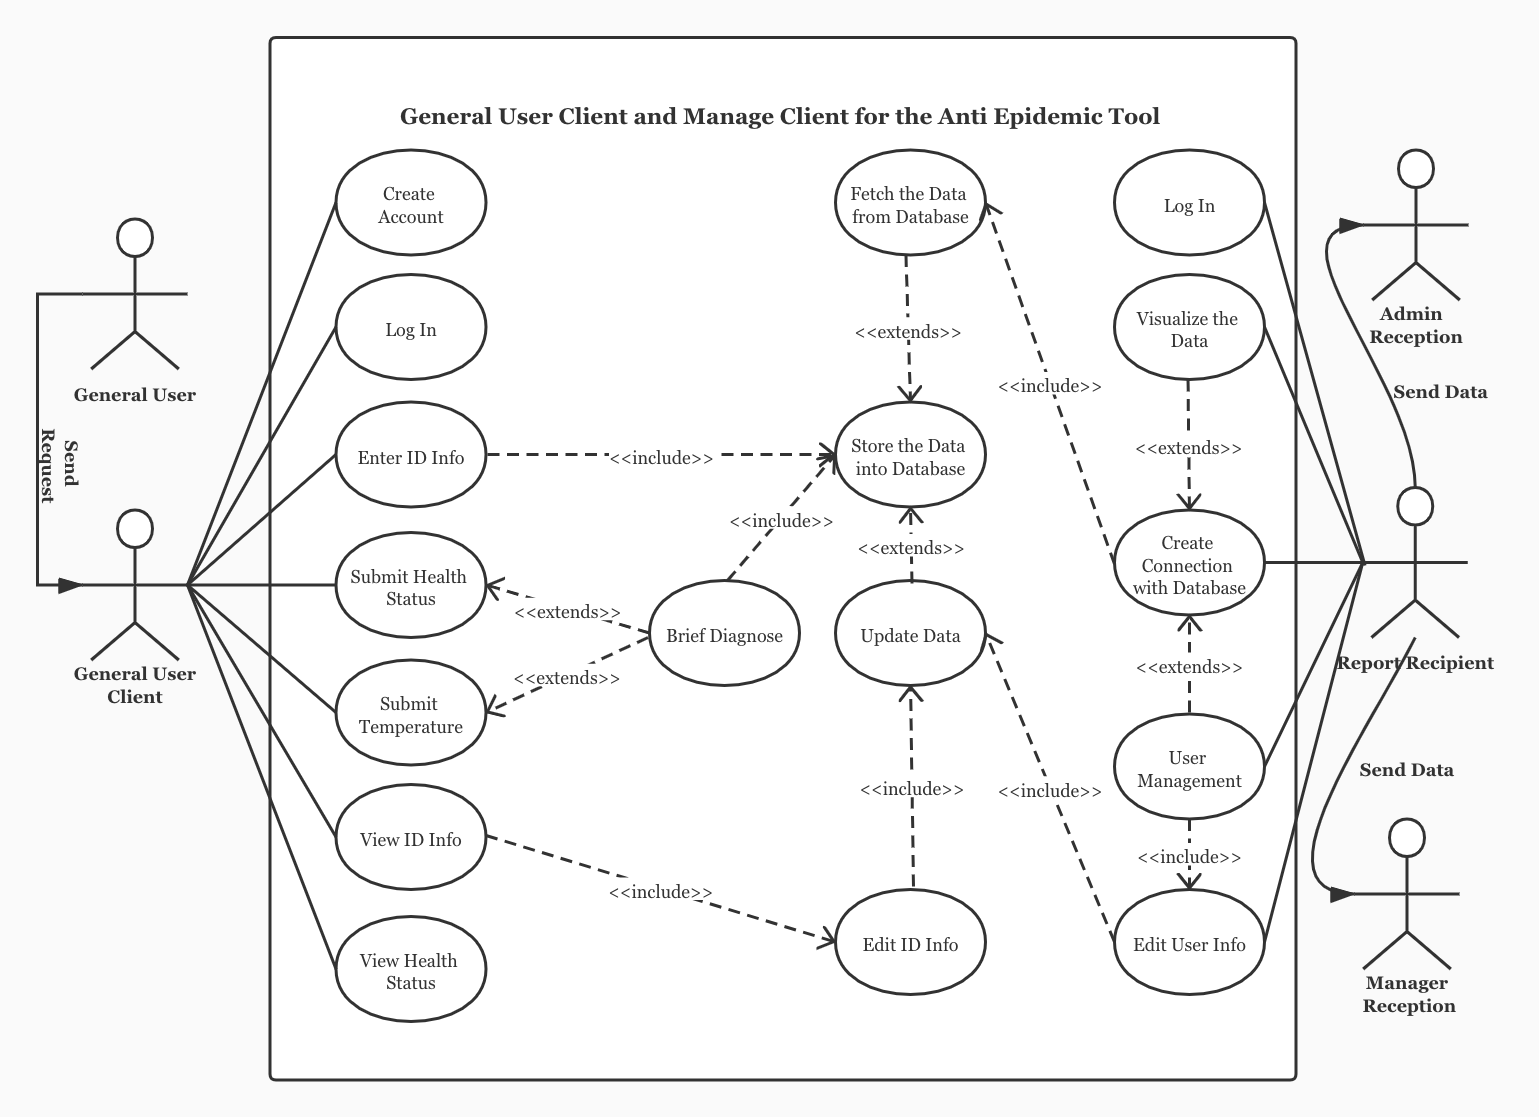
\includegraphics[scale=0.25]{ucd.jpg}
\caption{The Use Case Diagram for the System.}
\label{fig:label}
\end{figure}
\begin{itemize}
\item\textbf{Actors}
\\Actors are indicated as the users that will interact with the system. An actor is not necessarily always be a single person, it can also be an institution, a group, or someone, something will interact with the system.
\item\textbf{Use Case (System Function)}
\\A use case indicated a specific function that the system will perform, which task it will complete, the relation between system and actors, and how these functions will interact with actors.  
\item\textbf{Communication Link}
\\A solid link will connect an actor with a use case that indicates the connection and interaction between each other. Each actor must link with one or multiple use cases, but some use cases may not link to an actor. Where several arrow dotted lines communication links notated with ``extends'' that indicate the extended relationships between two use cases, the tip of the arrow dot line points to the parent use case and the tail of the dotted line connect with the child use case, which means the child use case extends from the base use case as an extension. Similarly, the arrow dot line notated with ``includes'' indicates the include relationships between two use case, in include relationships, the tip of the arrow dot line points to the child use case, and the tail of the dotted line will connect with the parent use case. A use case with additional functionality derives from the parent use case always indicated with include relationships in order to reuse the base functionality.
\end{itemize}
\subsection{Prototypes and UI Design}
As mentioned in the literature review, a reasonable user interface design will reduce the study cost, increasing usability. The UI design should apply the re-use concepts to let the user familiar with and keep the design style in the same theme both in the general user client and the manage client, to make them integrate. It also makes sense to keep the button and portal as concise and clear as possible when it does not affect the functionality and aesthetic as the first demand. 
\begin{itemize}
\item\textbf{General User Client}
\\The following figure 2 and figure 3 show the mockup of a user interface for the main features of the general user client. The prototypes were designed based on the traditional web browsers (IE, Chrome, Firefox) as a web application. Where there are three tabs at the left side of the page, The Current Status tab first represents the virus incubation period for the advice isolated days in order to observe whether the user has infected or not, the health status represents how likely that the user was been infected, give a suggestion whether need medical help, all of these are based on the last data submission from the user, on the basis of the body temperature and the symptoms that the user selected, the system will give corresponding advice and health status based on the different combination of body temperature and symptoms. At the bottom of the page are the notifications and news area, which will leave this part to update several latest news about the epidemic or advice about how to prevent the virus infection from the epidemic.
\\
\\In figure 3 is the page that the users that will submit the information about their daily health status, will enter in their current body temperature, and select their symptoms that showed up (Note: there will be a choice if the user feels well without any symptoms in the real implementation, if this choice has been selected, then other choices can not be selected, vice versa.), then they need to choose a city that they stay in last 14 days, the reason that needs the information about city stay in last 14 days is that according to the medical institutions, the virus incubation period for coronavirus is usually 14 days, therefore, collect this data will help the further data statistics to filter out which city may have a higher probability to be infected.
\\
\\The last tab will provide development info, guidelines or add new features in the future update. There will be more screenshots of UI design for the real implementation can be found in the appendix section.
\\
\begin{figure}[ht]
\begin{minipage}[t]{0.45\textwidth}
\centering
\includegraphics[scale=0.45]{user1.png}
\caption{Mockup UI a.\label{fig:1}}
\end{minipage}
\qquad
\begin{minipage}[t]{0.45\textwidth}
\centering
\includegraphics[scale=0.45]{user2.png}
\caption{Mockup UI b.\label{fig:2}}
\end{minipage}
\end{figure}
\item\textbf{Manage Client}
\\Figure 4 and figure 5 show the prototypes of the manage client where figure 4 indicates the UI of the user manage function, all the data collected from the general user client will be synchronized and demonstrate on the page of figure 4 separately. Also, in order to keep the system consistent, on the left side of the page, there are several tabs to let the managers switch different functions between user manage and data statistics function.
\begin{figure}[ht]
\begin{minipage}[t]{0.45\textwidth}
\centering
\includegraphics[scale=0.45]{manage1.png}
\caption{Mockup UI c.\label{fig:1}}
\end{minipage}
\qquad
\begin{minipage}[t]{0.45\textwidth}
\centering
\includegraphics[scale=0.45]{manage2.png}
\caption{Mockup UI d.\label{fig:2}}
\end{minipage}
\end{figure}
\\Figure 5 shows the data statistics function of the system, the aim of this function is trying to help the manager to filter out the most interesting or meaningful data quickly and visualize those data as a chart in order to observe the features of the data and doing further data analysis. 
\\
\\The algorithm of filter data will mainly be based on the decision of filter criteria and target, as the progress of the system development, more different filter criteria will be added in order to help the manager to do the data analysis in multiple aspects. There are more screenshots and figures of UI design for the managed client also can be found in the appendix section.
\\
\\In the next part, the detail of system architecture and application implementation will break down into small pieces and describe them in sequence.
\end{itemize}
\section{Architecture and Implementation}
\subsection{Architecture Design Overview}
First, let us recap how the cycle of this system will work. At the start, from a general user client, if users do not have an account yet, they need to register for one, after they finish the register, the new username and password pair will send to the database via a server, at the login procedure, the client will try to match the username and password pair with the database pre-stored, if the match is successful, users will be able to log in. Then the users can be able to use the functions of the application, if users want to send data, the data will go through with the server, the server will connect with the database and update the data from the client eventually. 
\begin{figure}[ht]
\centering
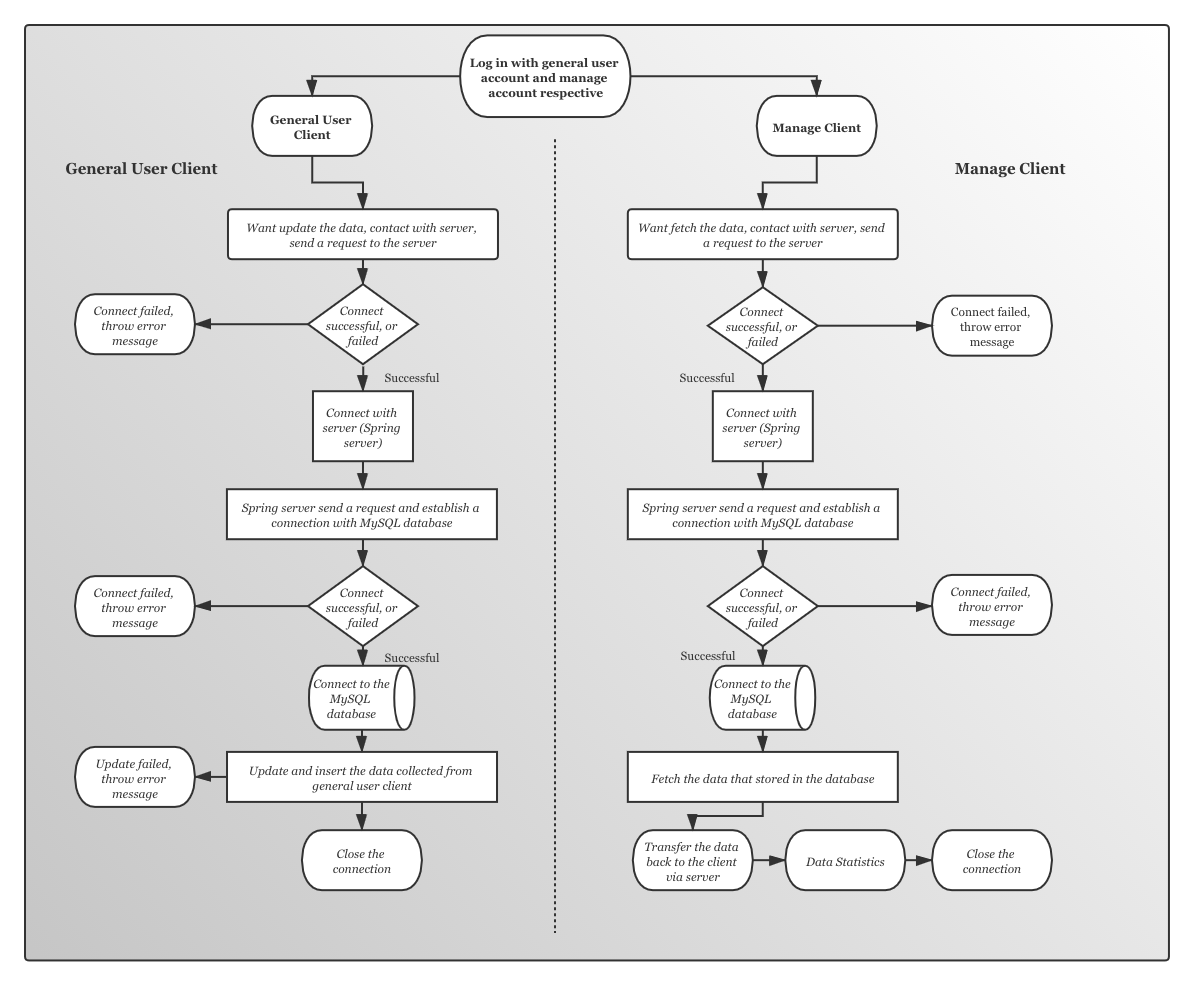
\includegraphics[scale=0.32]{flow.png}
\caption{The General Flowchart for the System.}
\label{fig:label}
\end{figure}
That is how the system work on the general user client, as the same scenario for the manage client except register an account, because, in this application, the register function for the manage client will be disabled, it is not allowed to register a manager account in this system at the initial design. After successfully log into the manage client, the client needs to fetch the data from the database, first, send a request to the server, then the server will establish a connection with the database, and the database will take all the necessary data send it back to the client via server. Figure 6 shows the flowchart for the entire system, generally, the system includes multiple small components, they interact with each other behind the system while the application is running in order to complete the task. The next couple of parts will explain those components and how to implement them in detail.
\subsection{System Components}
\subsubsection{Techniques for Implement the System}
The programming language that writes for the logic; back-end part is using ``Java 15.0.1'' with ``Java SE Runtime Environment build in 15.0.1+9-18'', using ``Java'' will be more convenient to interact with MySQL database by using Java Data Base Connectivity (JDBC). The UI; front-end part is implemented by using HTML, CSS, and JavaScript as a popular technique for web-pages design.
\subsubsection{Spring Framework}
The ``Spring Framework'' is an open-source framework that aims to reduce the complexity of software development. The key features can be applied by any java based application, there are several features that will be helpful while developing this application such as the IoC (Inversion of Control) container which allows the application to use a container to control the dependence between each class, function in java; ``The Data access framework'' will allow us to use APIs in the database, such as JDBC for storing the data also deal and reduce the various problems in the developing, for example, establish the connection and interact with the database, close the connection after each data transaction process has finished, deal with exceptions in the database management; ``The Spring MVC framework'' will allow the developer to build web applications based on MVC architecture; `` The Spring Web Service'' which will provide us a web service endpoints based on Java classes. In summary, ``Spring Framework'' includes a bunch of useful packages, APIs that will help developers to build a java application. Therefore, to enhance the implementation efficiency, several features from the ``Spring Framework'' will be applied.
\subsubsection{Database Schema}
As mentioned in the literature review and previous sections, MySQL will be the database management system used for this application to store the data. MySQL database always structured with tables, columns, and rows, the tables decide which kind of the data will store in the different tables, the data has stored in the same table often have relations with each other, a database usually constructs with several tables; each column represents a set of data values as a field in the database, a table usually construct with several fields; each row will record and store the data for each field. To present the relationship between each table and the construction of a database usually called a database schema. To build a database for this application, the following tables and fields will be defined:
\begin{figure}[ht]
\centering
\includegraphics[scale=0.2]{ds.jpg}
\caption{Database Schema of the System.}
\label{fig:label}
\end{figure}
\\Table ``admin account'' will store the admin account number and the password; table ``user'' will store the user's personal information including the username and password; table ``symptom'' will store the main symptoms of coronavirus; table ``status'' will store the general user current health status; table ``record'' will store the daily health data that submit from the user. A unique field was defined as the primary key in each table in order to link to other tables.
\subsubsection{Account Register and Login}
When the users are using this application, the first function that they contact with will be the register function if the users do not have an account yet or they need to log in to the system if they already have an account. By using ``\textit{\textbf{register}}'' function and transfer the new ``\textbf{username}'' and ``\textbf{password}`` via server and store the data into the database, the client needs to send a ``HTTP Request'' to the server in order to transfer the data between the client and the server. The following snippet code is method for the function ``\textit{\textbf{register}}'' first send a request to the server:
\\\textit{\textbf{@RequestMapping(method = RequestMethod.\textcolor{magenta}{POST})}}
\\\textit{\textbf{JSONObject data = \textcolor{cyan}{new} JSONObject(dataJson)}}
\\
As we can see from the code that uses the ``HTTP post'' method to send the data sourced from register pages to the server in order to process those data. Where ``\textit{\textbf{RequestMethod}}'' is packaging method from ''Spring'' for send requests to the server. After that, a ``JSON Object'' data structure will be created in order to store the data, in this case, it will store the ``\textbf{username}'' and the ``\textbf{password}''. Then for the new user, it is necessary to allocate the data attributes and space for the new account in the database, by doing this, it first need to connect with MySQL database via spring server, using the ``\textit{\textbf{jdbcTemplate.update}}'' and ``\textit{\textbf{createPreparedStatement()}}'' functions to create preparedstatement method in order to allocate the resource for the new user account to insert the data into the database. Using traditional preparedstatement MySQL grammar ``\textit{\textbf{INSERT INTO user(username, password) VALUES (?,?)}}'' to insert the new ``\textbf{username}'' and ``\textbf{password}`` into the database. Using preparedstament rather than statement will improve the readability of the code, enhance the execution efficiency and prevent the SQL injection attack. For the user Login, the application will use the same manner by sending a ``HTTP Request'' using post method to server; compare the username and password that pre-stored in the database by using MySQL query grammar ``\textit{\textbf{SELECT * FROM user WHERE username = ? AND password =?}}'', if the username and password are matched, then the server will give authentication to approve user log in and send it back to the client, thus, the user will be able to perform further operations.
\subsubsection{Data Collection from User}
After users have been successful login with general user client, data need to be collected from users in order to satisfy the functional requirements for this application. Those data can mainly divide into two parts:
\begin{itemize}
\item\textbf{General User Information}
\\This indicates the data of personal depend on the different users such as their name, gender, date of birth, ID number, etc the reason for collect those data is to recognize and distinguish each user. When the user types in and submit their personal information, the client will first send a request to the server for transfer the data to the database via the server: 
\\ \textit{\textbf{@RequestMapping(value = \textcolor{cyan}{``/submitUserInfo''}, method = RequestMethod.\textcolor{magenta}{POST})}}
\\In this case the data transfer to the server from the URL ``\textit{\textbf{submitUserInfo}}'' which is the initial webpage for users to enter their personal information. After send a request to the server, the server will connect with database by using ``\textit{\textbf{jdbcTemplate.update}}'' function, and MySQL grammar ``\textit{\textbf{UPDATE}}'' to update the personal information data that stored in the database.
\item\textbf{Daily Health Status}
\\This indicates the data that the user will submit each day such as the symptoms and body temperature, city that stay in 14 days. There are two usages for collect those data, the first is the latest data will store in the database so the manage client will fetch those data to do the further data statistics and analysis as mentioned in the functional requirements, the second usage is based on the symptoms and body temperature, the application will inside perform an algorithm to give a response to the user as mentioned whether the user needs medical help and give a result of the user current health status, whether healthy or not. As usual, the data will be updated in the same manner only change the link address.
\\ \textit{\textbf{@RequestMapping(value = \textcolor{cyan}{``/submitUserRecord''}, method = RequestMethod.\textcolor{magenta}{POST})}}
\end{itemize}
\subsubsection{Diagnose Algorithm}
A distinctive function that implemented in the general user client is when a general user enters the body temperature and select the symptoms provided, based on the answers from the user and the combination between body temperature and symptoms, the system will give a judgment that diagnoses whether the user currently might need medical help or not then send a response to the general user, and record such data into the database. 
\\
\\\textbf{NOTE: The algorithm and the diagnosis result aims to give the suggestions to the user and based on the common symptoms of the diseases in order to help the user to make the decision in some way, it is not hundred percent guarantee to determined that the user has been infected or not unless doing standard virus test or take the professional medical diagnose.} 
\\
\\Basically, the algorithm has four stages, 1. classify the body temperature; 2. classify the symptoms; 3. combine them and based on the different combinations give the final result. 4. client sends a response to the user. 
\begin{itemize}
\item\textbf{Classify the Body Temperature}
\\First, the algorithm divides the data of body temperature into two categories, ``\textbf{Normal}'' and ``\textbf{Fever}'', ``Normal'' indicates the body temperature is the common healthy body temperature range as we usually counted in, ``Fever'' which means the body temperature is beyond the range of health and fever is always a usual symptom in the coronavirus. The thresholds set of body temperature for the coronavirus is ``\textbf{37.3 }centigrade'', the temperature is lower than 37.3 will be classified into the category ``\textbf{Normal}'', rest will be classified into ``\textbf{Fever}''.
\item\textbf{Classify the Symptoms}
\\Then the algorithm will handle the symptoms that chosen from users. The symptoms will be divide into three categories, ``\textbf{Healthy}'', ``\textbf{Mild Symptoms}'', and ``\textbf{Serious Symptoms}'', in the real application implementation, there will be an option ``\textbf{All well without bad feeling}'' setup for users, users who select this option will be classified into category ``\textbf{Healthy}'', rest of the options are picked from common symptoms of coronavirus, some of the symptoms are classified into the ``\textbf{Mild Symptoms}'', others are classified into the ``\textbf{Serious Symptoms}'' when the users submit the result, the algorithm will count the total number of symptoms been chosen from ``Mild symptoms'' and `` Serious Symptoms'' then record them separately.
\item\textbf{Combine and Output the Result}
\\This step will calculate the final result, the algorithm will combine the results that acquired from body temperature section and symptoms chosen section in order to give the final result. Before state each result, the name of categories will be write in abbreviated as follow:
\\ ``\textbf{Normal}'' into ``\textbf{N}''; ``\textbf{Fever}'' into ``\textbf{Fe}''; ``\textbf{Healthy}'' into ``\textbf{Hea}''; ``\textbf{Mild Symptoms}'' into ``\textbf{MS}''; ``\textbf{Serious Symptoms}'' into ``\textbf{SS}''.
\\
\\Here each attribute will be assigned a weight(\textbf{w}) in order to calculate the final result that should point to. The rules of assign the weight defined as follow in the algorithm:
``\textbf{N}'' will be assigned ``0'' weight; ``\textbf{Fe}'' will be assigned ``0.5'' weights;
``\textbf{Hea}'' will be assigned ``0'' weight; ``\textbf{MS}'' will be assigned ``0.2'' weights; ``\textbf{SS}'' will be assigned ``0.3'' weights. Also, there are special cases are existing such as the user has already done the virus or PCR test and got the result or the user is included in the asymptomatic carrier, in such cases, if the test result was negative then the algorithm will treat the user as healthy and return to the result of healthy directly without doing the weighted arithmetic first, as the same idea, if the test result was positive or the user is an asymptomatic carrier, then the algorithm will handle the user as infected with virus situation directly. 
\\
\\There are mainly four different final results that will be point to: 1.``\textbf{Unlikely to be infected with isolation ended}''; 2.``\textbf{Unlikely to be infected, keep observe}''; 3.``\textbf{Likely to be infected, keep observe}''; 4.``\textbf{High likely to be infected, keep observe}''.
\\
\\After each submission, the algorithm will calculate the total weights based on the temperature(\textbf{T}) and symptoms(\textbf{S}) that user submitted, if the total weight is less than 0.5 and the remaining isolation day(\textbf{RD}) is not equal to 0, then the final result will point to ``Unlikely to be infected, keep observe'' and the remaining isolation day will reduce one day. This is the first case, other different cases for this algorithm are list as follow in general:
\begin{itemize}
\item\textbf{Case 2}
\\If $\mathbb{R}\in T$ and $s \in S$ (s indicate the different symptoms that stored) where total weights $\sum w < 0.5 $ and $RD = 0$ then the final result point to ``Unlikely to be infected with isolation ended''.
\item\textbf{Case 3}
\\If $\mathbb{R}\in T$ and $s \in S$ where total weights $\sum w \geq 0.5$ but $\leq 1$ then the final result point to ``Likely to be infected, keep observe'' and set the current remaining isolation day(RD) back to $RD = 14$.
\item\textbf{Case 4}
\\If $\mathbb{R}\in T$ and $s \in S$ where total weights $\sum w > 1$ then the final result point to ``High likely to be infected, keep observe' and set the current remaining isolation day(RD) back to $RD = 14$.
\end{itemize}
The final result which points to the ``\textbf{Unlikely to be infected with isolation ended}'' or ``\textbf{Unlikely to be infected, keep observe}'' will keep the isolated time count down as usual. On the other side, the final result which points to the ``\textbf{Likely to be infected, keep observe}'' or ``\textbf{High likely to be infected, keep observe}'' will reset the isolated time back to 14 days until meeting the requirements for the count down once again. The data generates from the algorithm (eg the final result of health status and the remaining time of isolation) will also be recorded into the database and transfer via the server to provide the data for the manage client.
\item\textbf{Responsive Window}
\\After users submit their options,  the client will output a responsive window to the user aims to give some suitable suggestions to the user. These different suggestions are various and also based on the different symptoms that user selected beside the final diagnose result from the algorithm. For example, if the symptoms selected from users are mainly including in respiratory diseases (eg cough, difficult breathing), but not meet the requirements of infected with coronavirus then the suggestion will be given from the view of respiratory illness treatment. Different responsive UIs can be found in the appendix section.
\end{itemize}
\subsubsection{Manage Client}
As mentioned previously, the manage client is use to manage and view data that stored in the database directly rather than first type the SQL query grammar manually if the manager or the administrator wants to search specific data. The manage client will fetch all necessary data based on the requirements as long as the data was stored in the database, the data transfer method is almost the same as before, first use ``HTTP post'' method to send a request then fetch the appointed data into the server by using MySQL query grammar. An example to access the data of temperature distribution as follow:
\\ \textit{\textbf{@RequestMapping(value = \textcolor{cyan}{``/getTemperature''}, method = RequestMethod.\textcolor{magenta}{POST})}}
\\ \textit{\textbf{SELECT temperature,count(*) num FROM record GROUP BY temperature;}}
\\So far, the data of temperature has been accessed, the next work is how to let the managers view those data when they actually use the client. As a web application, the natural way to write the user interface also we could call it front-end is by using language combined with HTML, CSS, and JavaScript to write a usable, elegant interface for web browsers. To fetch the data into the web page in order to get the resources and confirm the information will be shown correctly on the web page, it still uses the ``HTTP post'' method as usual to access indicate address of each data, the full steps defined as follow:
\\\textit{\textbf{\textcolor{magenta}{type}:\textcolor{cyan}{`post'},}}
\\\textit{\textbf{\textcolor{magenta}{url}:\textcolor{cyan}{`/getTemperature'},}}
\\\textit{\textbf{\textcolor{magenta}{dataType}:\textcolor{cyan}{`json'},}}
\\\textit{\textbf{\textcolor{magenta}{data}:\textcolor{magenta}{JSON}.\textcolor{yellow}{stringify}(json),}}
\\\textit{\textbf{\textcolor{magenta}{contentType}:\textcolor{cyan}{`application/json'},}}
\\Now the data of temperature has fetched into the web page, we can write the interface to define how to demonstrate the data to let the web page looks more good and beautiful. The rest of the data stored in the database can be fetched and implement recursively by using the same methodology.
\\
\\After finish collected data from general user clients, it is possible to predict and observe the trend of the epidemic. As an example, for the total number of students study in a specific course ``\textbf{$T_c$}'', give the number of students who have the symptoms of coronavirus or already infected ``\textbf{I}. It is likely to calculate the potential percentages of the students be infected will coronavirus ``\textbf{P = I/$T_c$}''. The client will also integrate the data and it much easier to compare data results from different aspects to help the University staffs and managers to comprehend the general status of the students.
\subsection{Front-end Implementation}
The idea of front-end design is generally followed the user interface design in section 3.4, during the implementation, some web UI frame has applied, the reason is that design the UI features from scratch is usually time-consuming and the result of the design always need to make a lot of corrections. Therefore, a web UI frame called ``\textbf{Layui}''  has implemented while writing the front-end. This web UI frame is an open-source project used to solve the web UI problem and totally followed the development rules of original HTML, CSS, and JavaScript. ``Layui'' was the main theme of the front-end design pattern of this application. Most of the designs including interaction buttons, tab controls, response windows, icons, color are implemented from ``Layui''. 
\\\textit{\textbf{$\mathbf{<}$script type\textcolor{cyan}{=`text/javascript'} src\textcolor{cyan}{=`../static/js/layui.js'}\\$\mathbf{><}$/scripts $\mathbf{>}$}}
\\\textit{\textbf{$\mathbf{<}$link herf\textcolor{cyan}{=`../static/js/css/layui.css'} rel\textcolor{cyan}{=`stylesheet'} \\type\textcolor{cyan}{=`text/css'}/$ \mathbf{>}$}}
\\Where above functions are use for load the ``Layui'' base frame, method ``\textit{\textbf{script type}}'' is first defined the type of this script is a javascript, then use method ``\textit{\textbf{src}}'' to load the external script file ``layui.js'' which include necessary scripts for the frame. Method ``\textit{\textbf{link herf}}'' is to access ``layui.css'' file for fetching the resources such as theme color, icon design that stored in. Finally, call method ``\textit{\textbf{rel}}'', ``rel'' is the abbreviation of the word ``relationship'' which defined the relationship between the current web page and the file that previously linked with to make sure every element can be shown properly.
\\
\\In the manage client, there is a function that implemented for doing the data statistics and outputs the result then draw the statistical charts, to draw the charts, a library called ``\textbf{ECharts}'' was implemented. ``ECharts'' is an open-source web-based visualization library wrote by JavaScript, it includes multiple statistical charts and diagrams in order to satisfy different requirements in application development. The function of histogram data statistics that implemented in the manage client is powered by ``ECharts''. To apply ``ECharts'', after importing the required packages and fetch the specified data into web page sources, invoke the ``ECharts'' as follow:
\begin{figure}[ht]
\centering
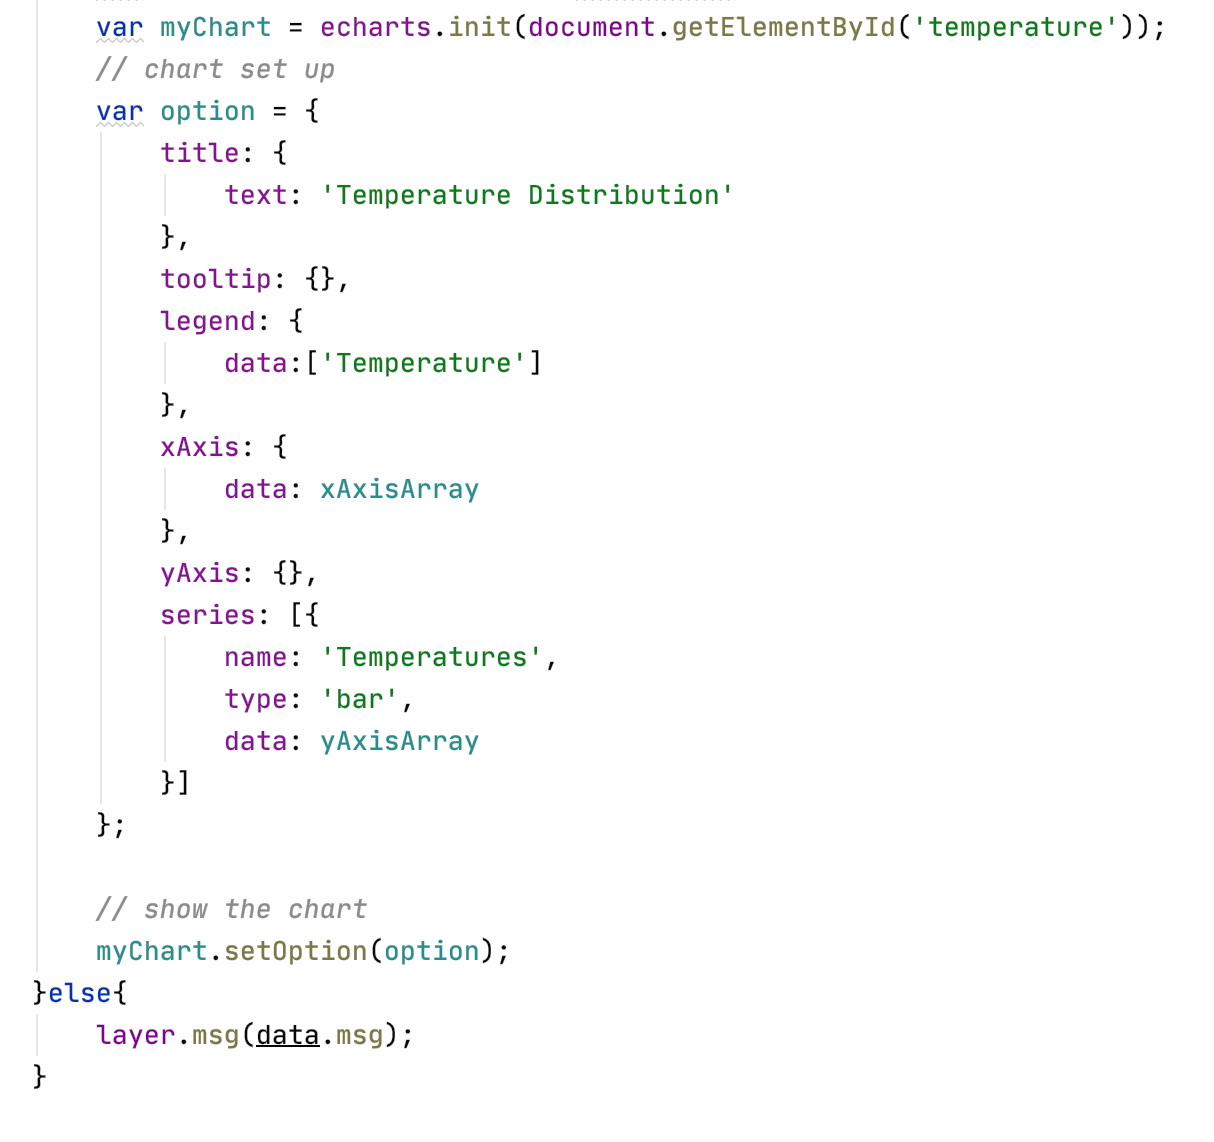
\includegraphics[scale=0.6]{pesudo.png}
\caption{The Functions for Invoke and Set Up the ECharts in order to Plot the Histogram of the Data of Temperature.}
\label{fig:label}
\end{figure}
\\The first line of the codes is to invoke and initialize the ``ECharts'' by calling the ``\textbf{echarts.init}'' function, then fetch the data. Under the function ``\textbf{option}'' are the methods to set up the components of the chart, the title, the data of x-axis and y-axis will be indicated, for the above example, a histogram will be plotted for the data of temperature. The application will support various statistics based on the data in the implementation, the design of the chart also can be found in the appendix section. 
\section{Test and Evaluation}
In the methodology section, the requirements of the application were defined which help to clarify the design choice and the implementation procedure for the system. In order to evaluate this application, in this part by first make a comparison with the general requirements and similar products to figure out the achievements of this project. Then by apply several technical evaluation methods to test the performance and stability of this system in order to evaluate the non-functional requirements, from the result, it will give more considerable ideas on the general accomplishment and further improvement of this project.
\subsection{Comparison}
This section mainly focuses on whether the requirements have been satisfied, how much works have been achieved for the specific requirement, and the improvements for the certain requirements, then, by comparing with other similar applications to indicate the advantages and disadvantages between each product.
\subsubsection{Compare with General Requirements}
\begin{itemize}
\item\textbf{Functional Requirements Comparison for General Users}
\\$\mathbf{(FR1.)}$ The client must create a unique user id (UID) and generate a token to identify each user. Based on the implementation, the client will be able to create an ``UID'' and a token for each user. However, the usage of the token was not shown intensely since using user id is a suitable method for user identification, it is a reasonable idea to apply the token as further user verification and security check for the system.
\\
\\$\mathbf{(FR4.)}$ The client must have a portal to let users be able to submit daily health status. This requirement has been successfully implemented but options of the symptoms are lacking during the initial version of the application, it is possible to add more different choices when users submit their daily health status in the future patch update and it is also compulsory to add various check function properly in order to prevent ``software maliciously use'', for example, submit the same result with total weights less than 0.5 multiple times will eventually let the isolation days reduce to 0 at once.
\\
\\$\mathbf{(FR11.)}$ The client shall give the time counting notification for their remaining isolation days. This has been implemented just ``fine'', the remaining isolation days will be able to count down or reset based on the initial idea of the algorithm design. Even though the implementation has been finished and there is no critical error has been found, but there are lots of controversies during the development, for example, how to decide the initial isolation days, how to count down the isolation days in order to make sure it is fair to everyone, what if the users are getting bad cold rather than infected with coronavirus or what if the users are infected with coronavirus just with slightly symptoms then how to deal with this to make sure the count down of isolation time is fair. Moreover, it is really easy to face the risk of ``software maliciously use'' since implementing another various check function will spend extra development time also more and more institutions support the virus test and the vaccines are currently manufacturing. To summarize the benefits and disadvantages, even this requirement has been implemented, but the importance has been reduced as before based on the analysis and current epidemic situation.
\\
\\$\mathbf{(FR14.)}$ The client may display the history of the submission. This requirement has not been implemented but it is a considerable feature for a health application since the initial idea of this project is aim to self -diagnosis, report and record the result. Therefore, the priority of this requirement has been declined. This requirement will put on the list to add in the future update.
\\
\\$\mathbf{(FR15.)}$ The client may support register and log in with University email addresses, accounts in order to reduce the potential accounts management issues in the future. It is a good to integrate the accounts for a particular group, although this requirement has not been implemented yet, but it is easy and will not take too much time to implement, one of the easiest possible ways to achieve this is simply import accounts username and password and store them into the database.
\item\textbf{Functional Requirements Comparison for Managers}
\\$\mathbf{(FR4.)}$ The client must update and refresh the data after receive each new submission or update from the user client. Each time there are new data received, it will synchronize with the database without any data loss issues, but in order to view the latest data and result on the client, the manage client needs to refresh the web page manually first since there is no automated refresh mechanism have been implemented yet when there are new data flow received.
\end{itemize}
The rest functional requirements for both clients that not mentioned above are most successfully accomplished. Overall, the main goal and the major functionalities of this system have been achieved. 
\subsubsection{Compare with Similar Products}
\begin{itemize}
\item\textbf{Google Sheets}
\\Google Sheets is a famous application for data statistics developed by Google. The web version of Google Sheets is allow the user share with a public access link to let other users with this link have a permission to view and modify the file. The advantages of Google Sheets is stable with fully functional, it also has the fancy data statistics features by using charts and diagrams, there are less system errors will occur while using it. However, the personal privacy may leakage since everyone will access via the public link also can view the entire details that stored in the file, and if the user without a proper use the functions, it may modify other user's information, this may cause the data collection fault.
\item\textbf{WeChat Form Application}
\\This is a lightweight web application set up the platform of WeChat, this is also a typical way for users who are self-isolating in China to report their daily health status since WeChat is a popular usage application in Asia. This application allows users to access via WeChat and send the data to the backstage of the application privately, so this solved the problems of information leakage in a way.  But the features is lack and simple, it only allows the users to submit the basic information by typing for the record purpose without anything else. At the backstage of the application it also merely allowed to view those information that collected from the user without other functions such as data filter or statistics.
\end{itemize}
\subsection{Technical Evaluation}
To evaluate the non-functional requirements, first by using ``\textbf{Query Profiler}'' which is a debugging tool that assists with MySQL after version 5.0.37 for check the accurate execution time for each querying to make sure the performance is satisfied enough. Then write a ``MySQL script'' to add a vast number of testing data to test the limit of the database also to compare the performance difference when dealing with a large amount of the data.
\begin{itemize}
\item\textbf{Test the Performance}
\\To use the function of the MySQL debugging tool, by installed the MySQL command-line tool first, execute the standard querying function then use the command ``\textit{\textbf{show profiles}}'' which will show the total execution time for MySQL, moreover, not only for total execution time, it also support for various information check, as an example, use ``\textit{\textbf{show profile for query n}}'' to check execution time for a specific query or use ``\textit{\textbf{show profile for cpu; IO}}'' to check resource consumption for the query. The result of performance and resource consumption for 100 columns of data are represented as follow:
\begin{table}[h]
\centering
\begin{tabular}{|l|c|c|c|c|}\hline
Query&Shortest ET(s)&Longest ET(s)&Average ET(s)\\\hline
Select * From user&0.00019450&0.00021675&0.00020388\\
Set Extra Condition &0.00029850&0.00031075&0.00030190\\\hline
Select course From user&0.00016775&0.00019665&0.00017881\\
Set Extra Condition&0.00018125&0.00021100&0.00019698\\\hline
\end{tabular}
\caption{The Execution Time(ET) for MySQL Query.}
\label{tab:Margin_settings}
\end{table}
\\Based on the result from Table 1, in the small set of data, the execution time has fully met the non-functional requirements of time performance $\mathbf{(NFR4.)}$, also from the result can observe that query of the fields will affect the performance since use ``\textbf{*}'' will output all the data fields that stored, therefore, it needs more time to traversal and adds more conditions will increase the execution time to search. There are various factors that will affect the performance of the database such as network quality, hardware, memory usage may also slow down the speed. The full result of MySQL execution time can be found in the appendix section.
\item\textbf{Capability and Resource Consumption}
\\To test the capability of the database to make sure it still fully functional under a large amount of data, first by using a ``MySQL script'' to insert 10000 extra columns of test data recursively, insert these manually will take too much time. The idea to insert the test data is to use the mechanism of storage procedure, then write a recursive algorithm in it, the pros of this method is naive with clear logic and easy to use but the cons is may take a little bit more time to add the data since it used recursively. The pseudo-code indicates the basic idea for this script mechanism:
\\\textit{\textbf{1. DELIMITER 
\\2. DROP PROCEDURE IF EXISTS `procinsertdata'
\\3. CREATE PROCEDURE `procinsertdata'()
\\4. DECLARE data INTEGER DEFAULT 1;
\\5. WHILE data $< =$ 10000 DO 
\\6. INSERT INTO user VALUES
\\(data, CONCAT('test', data), data + 10);
\\7. SET data = data + 1;
\\9. END WHILE; 
\\10. END
\\11. DELIMITER;
\\12. CALL procinsertdata ();}}
\\This will take about 0.8 second to finish insert all the test data. However, depend on the CPU performance and memory usage, the speed will be slightly different.
\begin{table}[h]
\centering
\begin{tabular}{|l|c|c|c|c|}\hline
Query&Shortest ET(s)&Longest ET(s)&Average ET(s)\\\hline
Select * From user&0.00860350&0.00882050&0.00871179\\
Set Extra Condition &0.00873550&0.00910570&0.00885408\\\hline
Select course From user&0.00835120&0.00861255&0.00849133\\
Set Extra Condition&0.00865600&0.00885535&0.00876096\\\hline
\end{tabular}
\caption{The Execution Time(ET) for MySQL Query with 10100 Data.}
\label{tab:Margin_settings}
\end{table}
\end{itemize}
Without a doubt from table 2 shows the number of totals stored in the database will also impact the performance of the database since the number of the data has increased from 100 to 10100, although the execution time has been significantly increased due to the development of technology both in the hardware and network, this will still satisfied the non-functional requirements even with a large amount of data in the reasonable ranges.
\begin{table}[h]
\centering
\begin{tabular}{|l|c|c|c|c|}\hline
Execution Type&Duration(s)&CPU(user)&CPU(system)\\\hline
Sending Data (100 datasets)&0.00004500&0.000001&0.000001\\
Sending Data (Complex Query)&0.00015500&0.000001&0.000001\\\hline
Sending Data (10100 datasets)&0.00835000&0.025625&0.000001\\
Sending Data (Complex Query)&1.22755000&0.116550&0.024500\\\hline
\end{tabular}
\caption{The Duration and CPU Usage for Sending Data.}
\label{tab:Margin_settings}
\end{table}
\\The total execution time for each query can be split into small pieces to see each small operation in the execution of querying. During with total of 15 different operations (Appendix Table 8) to finish the query, sending data has taken up the most percentages of the execution time, also from table 3 shows the number of data stored in the database and the logic of the querying will affect the speed of sending data. For the single, non-complex querying, the CPU usage has no distinct fluctuation all the time. However, when test the limit of the performance, a complex, naive without any optimized query was designed, a test example using ``select * from table 1 to table 10 together'' with each table have more than 100000 different columns of data stored in it, after execute the querying, the CPU usage and memory occupy were significantly increasing, for the personal laptop it may have rare chance to let query crash.
\\
\\In general, the system has met most non-functional requirements, most of the time it will be able to deal with common, large datasets without any pressure under the current home use hardware, software techniques and equipment, however, in order to let the system deal with the exceeding size of the datasets in stable and reliable, by using high performance or industrial level hardware, software and server probability be a more considerable choice to apply with, also, optimizing the algorithm and logic arithmetic are still the important roles in the area of computer science since there are various factors will impact the system performance.

\section{Conclusion}
\begin{itemize}
\item\textbf{Discussion and Future Improvements}
\\The anti-epidemic application is consists of front-end and back-end separately, before starting this project, I had very limited knowledge about front-end programming and set up a server by using ``Spring Framework''. Thus, construct the architecture and how to connect with each component of this system from zero has spent substantial time before working on the real implementation. Though this application has met the initial expectation and the idea of this system has been demonstrated, but there still have some improvements that need to consider about in order to give the user a better user experience. One of the major points is lack of the features, for the general user client, the users can only submit and view very basic information of themselves, it is possible to implement new features such as users can view the submit history, and it can be able to do statistics about their daily health status on their own client. Or provide a ``make an appointment'' feature to let the user can reserve medical help via the application will be another way to let the application be more distinctive. For the manager client, it is better to use various methods to do the data statistics like pie charts and line charts for different data rather than only using histograms. Moreover, one or several machine learning algorithms could be implemented in the data statistics part in order to let the result of statistic analysis being more meaningful. 
\item\textbf{Epilogue}
\\This project has designed and implemented an anti-epidemic web application along with a data management system. The initial idea of this project was invented from the worldwide outbreak. Moreover, during the development, a couple of new thoughts came up. The first is to build an application from scratch is not always like only ``write the code with an idea'', doing study research first, from low-level architecture to high-level programming will always let the development yield twice the result with half the effort. The second is many health problems have been ignored or not handled properly due to lack of health care management, in the future, this application can be extended into a general healthcare application with the basic scenario remain the same to benefit the welfare system of different institutions in the future.
\end{itemize}
%TC:ignore
\newpage
\addcontentsline{toc}{section}{References}
\bibliographystyle{unsrt}
\bibliography{mybib}
\newpage
\addappheadtotoc
\section*{Appendix}
\appendix
\section*{A. The UI Design}
\begin{figure}[ht]
\centering
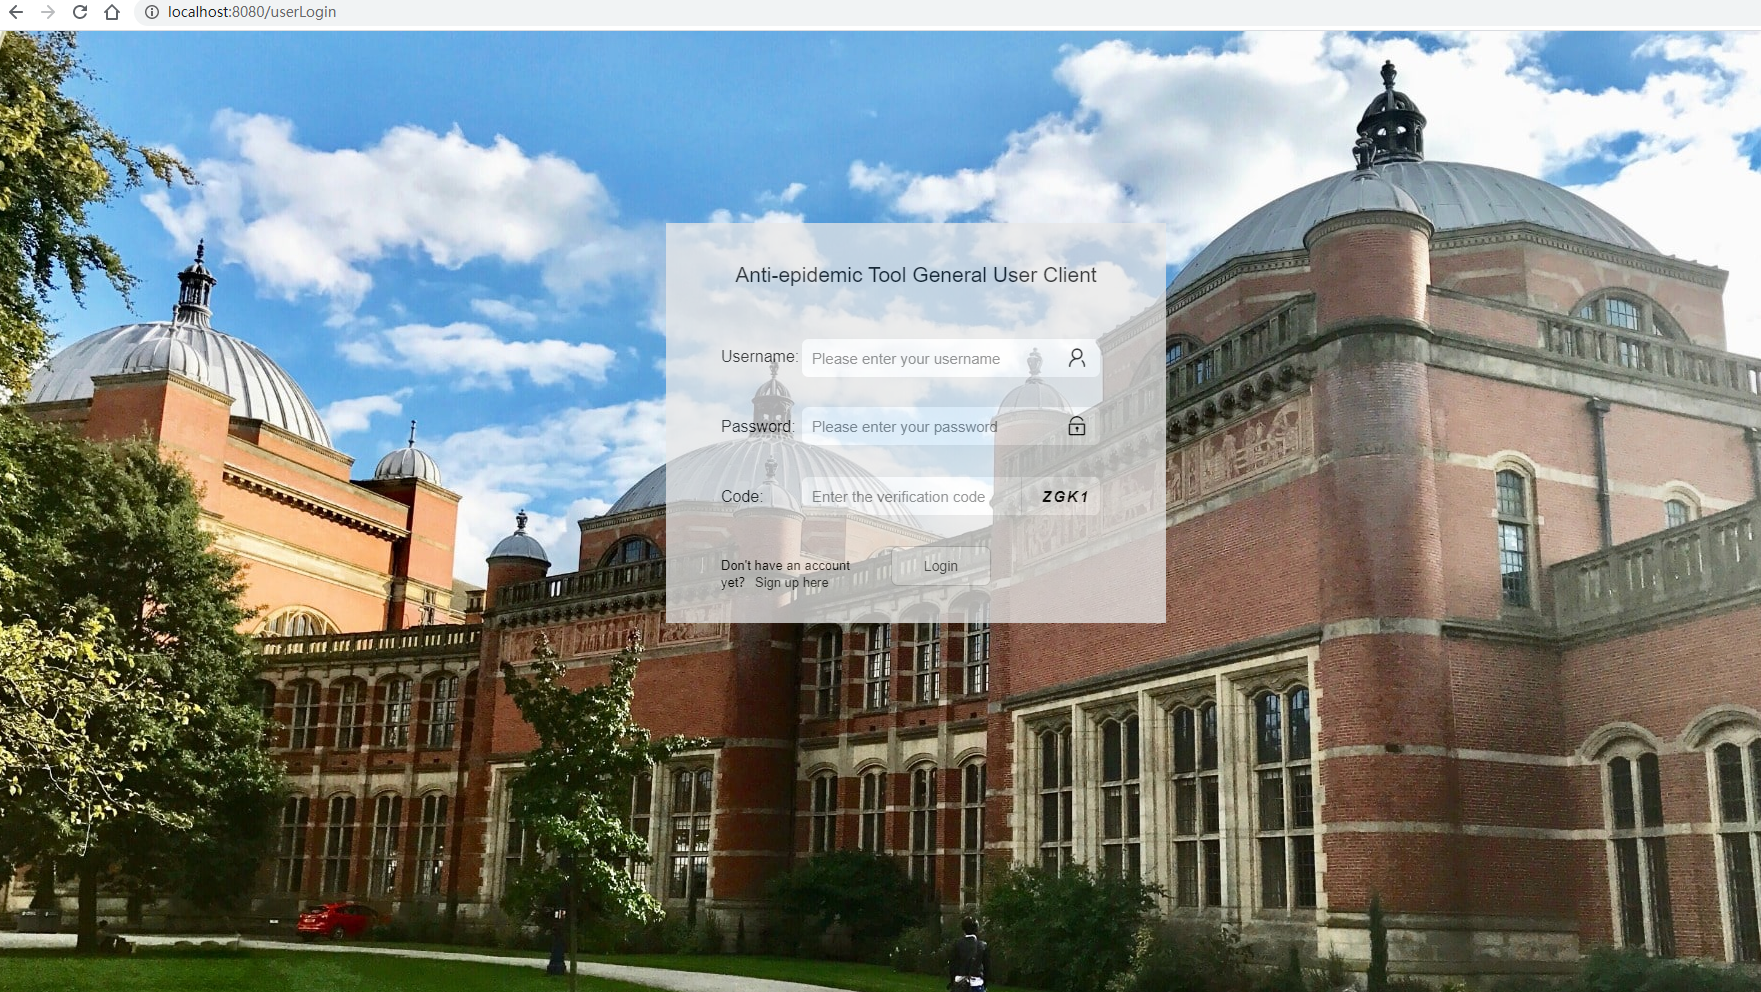
\includegraphics[scale=0.23]{ui1.png}
\caption{The Login Page.}
\label{fig:label}
\end{figure}
\begin{figure}[ht]
\centering
\includegraphics[scale=0.23]{ui2.png}
\caption{The Main Page after Login. Latest News Will Show Here.}
\label{fig:label}
\end{figure}
\newpage
\begin{figure}[ht]
\centering
\includegraphics[scale=0.23]{ui3.png}
\caption{The Report Page.}
\label{fig:label}
\end{figure}
\begin{figure}[ht]
\centering
\includegraphics[scale=0.4]{ui8.png}
\caption{Responsive Window a.}
\label{fig:label}
\end{figure}
\begin{figure}[ht]
\centering
\includegraphics[scale=0.4]{ui9.png}
\caption{Responsive Window b.}
\label{fig:label}
\end{figure}
\newpage
\begin{figure}[ht]
\centering
\includegraphics[scale=0.23]{ui7.png}
\caption{The Page for General User Update Information.}
\label{fig:label}
\end{figure}
\begin{figure}[ht]
\centering
\includegraphics[scale=0.23]{ui4.png}
\caption{The Main Page of Manage Client.}
\label{fig:label}
\end{figure}
\newpage
\begin{figure}[ht]
\centering
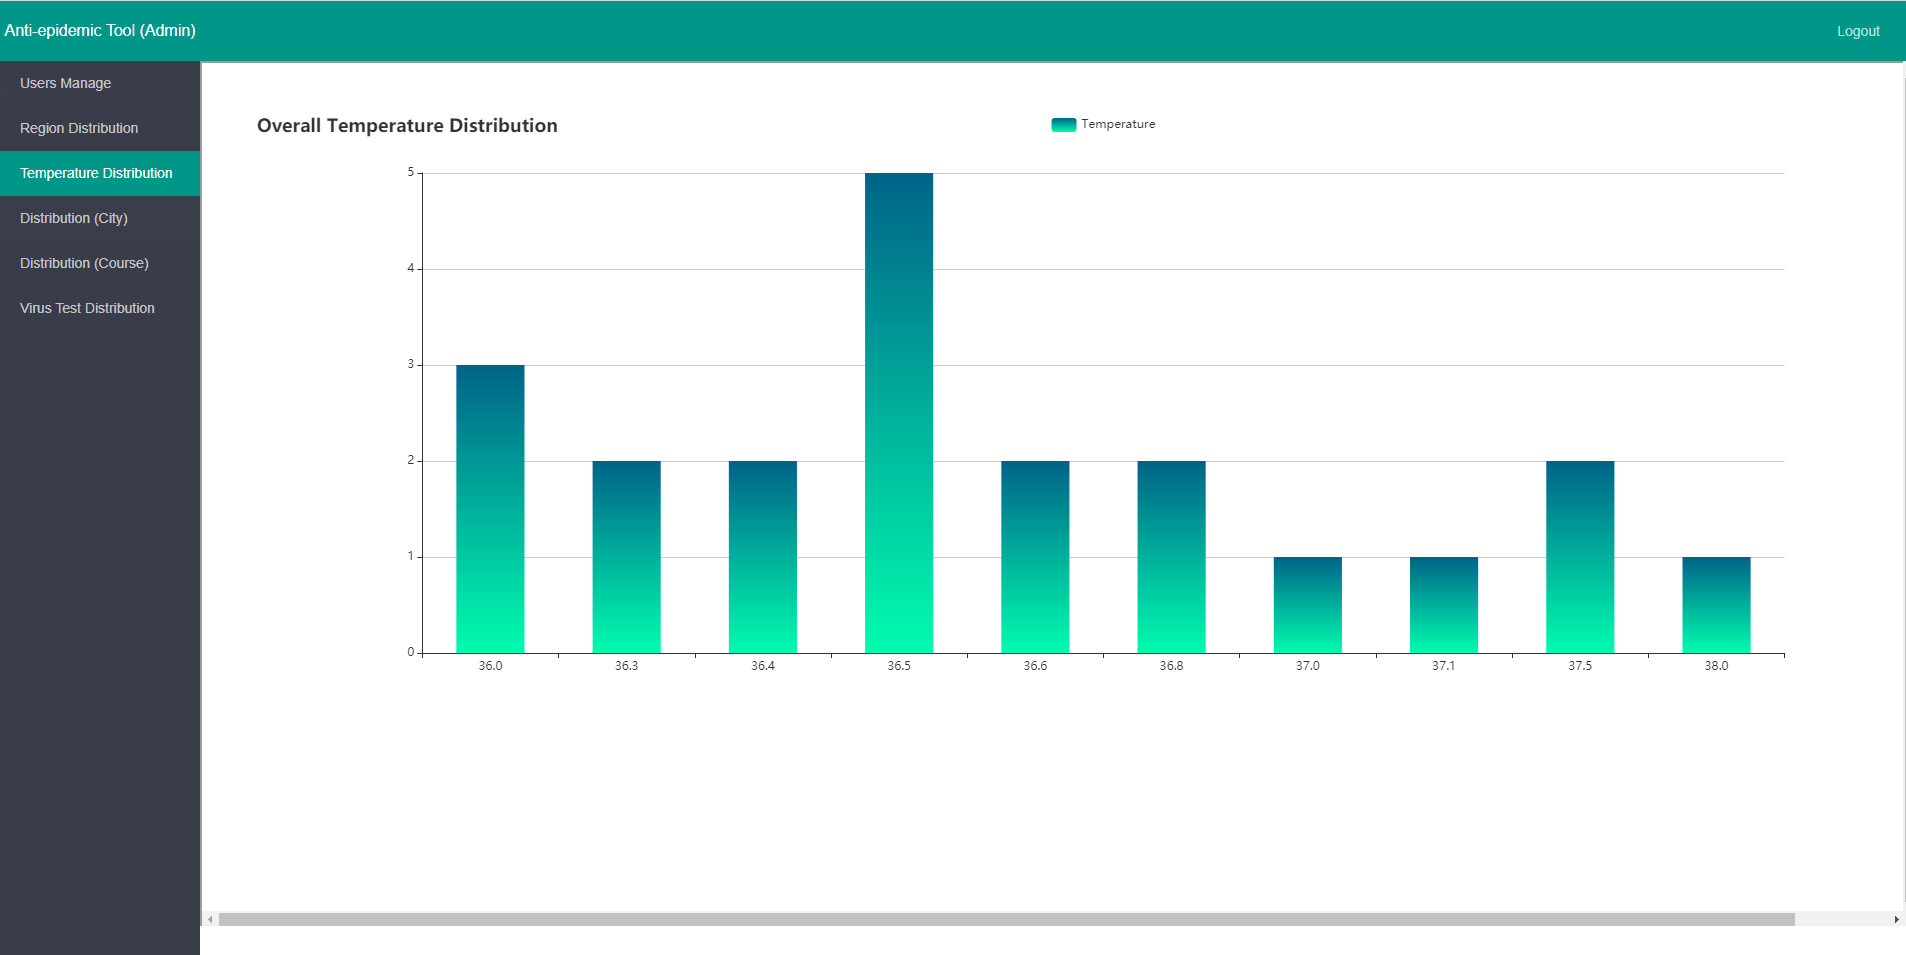
\includegraphics[scale=0.23]{ui5.png}
\caption{The Data Statistics Function of Mange Client a.}
\label{fig:label}
\end{figure}
\begin{figure}[ht]
\centering
\includegraphics[scale=0.23]{ui6.png}
\caption{The Data Statistics Function of Mange Client b.}
\label{fig:label}
\end{figure}
\newpage
\section*{B. The Execution Time Result}
\begin{table}[h]
\centering
\begin{tabular}{|c|c|c|c|c|}\hline
Result 1&Result 2&Result 3&Result 4&Result 5\\\hline
0.00020330&0.00019450&0.00020245&0.00019950&0.00019550\\
0.00029990&0.00029600&0.00029970&0.00031075&0.00030050\\\hline
0.00019350&0.00017700&0.00019665&0.00016850&0.00017750\\
0.00019620&0.00018125&0.00021100&0.00019550&0.00018700\\\hline
\end{tabular}
\caption{The Complete Result for Table 1 (First Half).}
\label{tab:Margin_settings}
\end{table}
\begin{table}[h]
\centering
\begin{tabular}{|c|c|c|c|c|}\hline
Result 6&Result 7&Result 8&Result 9&Result 10\\\hline
0.00020550&0.00021450&0.00020050&0.00021675&0.00020855\\
0.00030500&0.00030750&0.00029950&0.00030160&0.00029850\\\hline
0.00016775&0.00016950&0.00018650&0.00017555&0.00017560\\
0.00019710&0.00019125&0.00020200&0.00021000&0.00019850\\\hline
\end{tabular}
\caption{The Complete Result for Table 1 (Second Half).}
\label{tab:Margin_settings}
\end{table}
\begin{table}[h]
\centering
\begin{tabular}{|c|c|c|c|c|}\hline
Result 1&Result 2&Result 3&Result 4&Result 5\\\hline
0.00867230&0.00860660&0.00875500&0.00861450&0.00882050\\
0.00886500&0.00879550&0.00885000&0.00876550&0.00900505\\\hline
0.00836220&0.00860050&0.00845600&0.00835120&0.00855220\\
0.00876600&0.00878560&0.00883530&0.00875655&0.00885535\\\hline
\end{tabular}
\caption{The Complete Result for Table 2 (First Half).}
\label{tab:Margin_settings}
\end{table}
\begin{table}[h]
\centering
\begin{tabular}{|c|c|c|c|c|}\hline
Result 6&Result 7&Result 8&Result 9&Result 10\\\hline
0.00866535&0.00877550&0.00880500&0.00860350&0.00879965\\
0.00873550&0.00878500&0.00878800&0.00884550&0.00910570\\\hline
0.00836500&0.00859750&0.00861255&0.00841520&0.00860095\\
0.00867670&0.00879630&0.00880930&0.00865600&0.00867250\\\hline
\end{tabular}
\caption{The Complete Result for Table 2 (Second Half).}
\label{tab:Margin_settings}
\end{table}
\begin{table}[h]
\centering
\begin{tabular}{|c|c|}\hline
Status&Duration(s)\\\hline
Starting&0.000029\\\hline
Checking Permissions&0.000005\\\hline
Opening Tables&0.000012\\\hline
Init&0.000012\\\hline
System Lock&0.000005\\\hline
Optimizing&0.000003\\\hline
Statistics&0.000007\\\hline
Preparing&0.000006\\\hline
Executing&0.000002\\\hline
Sending Data&0.000050\\\hline
End&0.000003\\\hline
Query End&0.000004\\\hline
Closing Table&0.000005\\\hline
Freeing Items&0.000045\\\hline
Cleaning Up&0.000007\\\hline
\end{tabular}
\caption{The Complete Operations for Querying.}
\label{tab:Margin_settings}
\end{table}
%TC:endignore
\end{document}
